
\documentclass[fleqn]{report}
\usepackage{graphicx}
\usepackage{amsmath}
\usepackage{rotating}
\usepackage{fancyhdr}
\usepackage{longtable}
\usepackage{epsfig}
\usepackage{lscape}
\usepackage{boxit}

\pagestyle{fancy} \setlength{\headwidth}{6.2in}
\renewcommand{\chaptermark}[1]%
{\markboth{\MakeUppercase{\thechapter.\ #1}}{}}
\renewcommand{\sectionmark}[1]%
{\markright{\MakeUppercase{\thesection.\ #1}}}
\renewcommand{\headrulewidth}{0.5pt}
\renewcommand{\footrulewidth}{0pt}
\newcommand{\helv}{%
\fontfamily{phv}\fontseries{b}\fontsize{9}{11}\selectfont}
\fancyhf{} \fancyhead[LE,RO]{\helv \thepage} \fancyhead[LO]{\helv
\rightmark} \fancyhead[RE]{\helv \leftmark}
\setcounter{totalnumber}{9}

\newcommand{\JL}{L^J}
\topmargin -0.5in \oddsidemargin  0 in \evensidemargin  0 in
\textwidth  6.2 in \textheight 9 in \setlength{\parindent}{0.0in}
\setlength{\parskip}{7pt plus 1pt}
\newcommand{\tight}{\itemsep 0pt}
\newcommand{\code}[1]{{\small \texttt{#1}}}
\newcommand{\email}[1]{{\texttt{#1}}}

\sloppy
\begin{document}
\pagestyle{plain} \pagenumbering{roman}
%% $Id: title.tex,v 1.12 2001/08/18 00:56:25 borning Exp $
%% Title information

\title{An Extensible, Modular Architecture for Simulating Urban
Development, Transportation, and Environmental Impacts}
\author{Michael Noth}
\renewcommand{\thefootnote}{\fnsymbol{footnote}}
\setcounter{footnote}{0} \hspace{-7.5mm} \footnote{Corresponding
author}
%\renewcommand{\thefootnote}{\arabic{footnote}}
\author{Alan Borning}
\address{Dept.\ of Computer Science \& Engineering,
University of Washington, \\
Box 352350,
Seattle, Washington 98195,
\{noth,borning\}@cs.washington.edu}
\author{Paul Waddell}
\address{Evans School of Public Affairs,
University of Washington, \\
Box 353055, Seattle, Washington 98195,
pwaddell@u.washington.edu}

\renewcommand{\thefootnote}{\arabic{footnote}}
\setcounter{footnote}{0}

%\begin{tabular}{cc}
%Michael Noth and Alan Borning        &    Paul Waddell \\
%Dept.\ of Computer Science \& Engineering  & Evans School of Public Affairs \\
%University of Washington, Box 352350 &  University of Washington, Box 353055 \\
%Seattle, Washington 98195 &  Seattle, Washington 98195 \\
%\{noth,borning\}@cs.washington.edu  & pwaddell@u.washington.edu
%\end{tabular}
%}

%\maketitle

%{\large\bf\em Draft.}  \emph{We have submitted this paper for
%journal publication --- comments and suggestions are most
%welcome!}

% LocalWords:  noth Waddell Exp pwaddell Borning

%% $Id: acknowledgements.tex,v 1.1 2006/01/30 21:12:08 pwaddell Exp $

{\bf \large Acknowledgments}

The project described in this report has been funded principally
by the Puget Sound Regional Council. It was also supported by
grants from the National Science Foundation Grants CMS-9818378,
EIA-0121326 and EIA-0090832, which have supported the development
of UrbanSim.

Numerous people have contributed substantially to the development
of this report and the analysis it contains.  In particular, we
wish to acknowledge the support of Mark Simonson and Larry Blain
at the Puget Sound Regional Council, who coordinated the Technical
Advisory Committee. Considerable assistance was also provided by
Kevin Murphy, Jeff Frkonja, Carol Naito, Jerry Harless, Andy
Norton, Kristen Koch, Neil Kilgren, and others at the PSRC.
Members of the Technical Advisory Committee, listed below, were
instrumental in improving the database and providing valuable
feedback in this effort.  At the Center for Urban Simulation and
Policy Analysis, Chris Peak and Peter Caballero carried out much
of the database development effort, with considerable assistance
from Jack Kim, who analyzed non-residential real estate, Kapena
Pflum, who assisted in documentation and in verification of
employment, Liming Wang, who developed scripts for data
processing, Bjorn-Freeman Benson, Rob Duisberg and David Socha,
who developed key software components to facilitate the data
analysis and processing.

{\bf \large Center for Urban Simulation and Policy Analysis}

The Center for Urban Simulation and Policy Analysis (CUSPA) at the
University of Washington brings advanced research and information
technology to bear on complex social, economic, and environmental
problems in metropolitan areas.  CUSPA is committed to the
development and pursuit of an integrated long-term research agenda
to help understand and anticipate the consequences of policy
choices regarding transportation, land use, housing, community and
economic development, and environmental quality, and to enable
more effective development, implementation, and evaluation of
policies. CUSPA is equally committed to making this research
widely accessible to policymakers and communities through the
development of information technology for advanced simulation
modeling, visualization, and decision support to facilitate
informed and democratic community policy decisions that involve
uncertainty, complex interdependencies, and conflicts over values
and strategies.

CUSPA is structured as an interdisciplinary research center at the
University of Washington, drawing together expertise from across
the campus to address common challenges.  It engages in strategic
partnerships with public agencies to facilitate linking research,
application, and education.  In short, CUSPA attempts to bring the
best available research to bear on the most pressing urban and
environmental problems faced by metropolitan regions in the U.S.
and elsewhere.

\begin{tabbing}
Director: Director: Director: \= \kill Director:\> Paul Waddell,
Evans School of Public Affairs \\
Associate Director:\> Alan Borning, Computer Science and Engineering \\
Steering Committee:\> Marina Alberti, Urban Design and Planning \\
               \> Batya Friedman, Information School \\
\>Scott Rutherford, Civil and Environmental Engineering \\\\
Center Home Page: \> {\bf www.cuspa.washington.edu} \\
UrbanSim Home Page: \> {\bf www.urbansim.org}
\end{tabbing}

\newpage
{\bf \large Technical Advisory Committee} \\

Travis Black -- Kitsap County \\
Larry Blain -- Puget Sound Regional Council\\
Dan Cardwell -- Pierce County \\
Greg Cioc -- Kitsap County \\
Steve Cohn -- City of Bellevue \\
Chandler Felt -- King County \\
Lauren Giboney -- Snohomish County \\
Michael Hubner -- The Suburban Cities Association of King County \\
Tim Koss --Snohomish County \\
Kevin Murphy -- Puget Sound Regional Council\\
Scott Murphy -- Kitsap County \\
Carol Naito -- Puget Sound Regional Council\\
Jennifer Pettyjohn -- City of Seattle \\
Shawn Phelps -- Pierce County \\
Jason Rice -- Kitsap County \\
Mark Simonson -- Puget Sound Regional Council\\
Steve Toy -- Snohomish County \\
Lish Whitson -- City of Seattle \\

\newpage
%% $Id: overview.tex,v 1.17 2001/08/18 00:56:25 borning Exp $

\section{Overview of the UrbanSim Architecture}
\label{sec:overview}

To simulate an urban region, UrbanSim employs a collection of
interacting \emph{models}, representing different actors and
processes in the urban environment, such as residents, businesses,
land developers, and transportation networks.  Each model encodes
the behavior of agents in the simulation, as well as the objects
they operate upon, such as land parcels and buildings.  Objects
correlate directly with easily-identifiable objects in the real
world, making it easier to reason about their properties and
behaviors.  Agents can be shared across models, as can the objects
they operate upon.  Much more than other urban modeling systems,
the UrbanSim model is very disaggregate and has high data
requirements.  These requirements enable modeling of processes to
be done at a fine level, which allows use of detailed spatial data
in a manner not possible with more aggregate systems.  At the same
time, this makes the design and implementation of the system more
difficult from a software perspective.  Figure \ref{fig:USArch}
illustrates the software architecture of the UrbanSim system.

\begin{figure*}
\center \resizebox{0.75
\textwidth}{!}{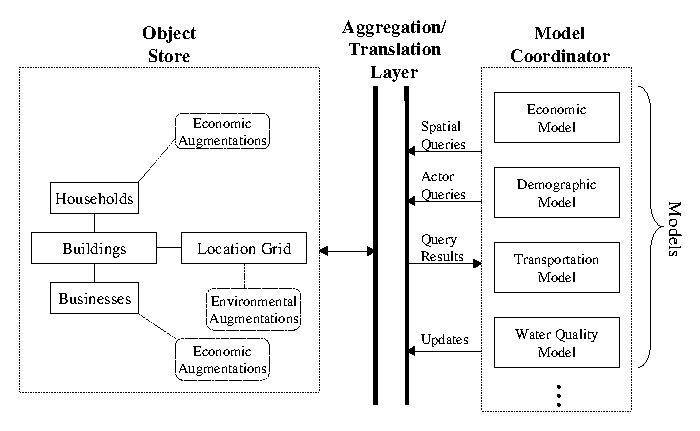
\includegraphics{USDiag1.eps}} \caption{UrbanSim
architecture} \label{fig:USArch}
\end{figure*}

%Figure~\ref{fig:USArch}: UrbanSim architecture.

In addition to the models, the other principal components of
UrbanSim are a \emph{model coordinator} that schedules models to
run and notifies them when data of interest have changed, an
\emph{object store} that holds the shared representations of
agents and other entities in the simulated world, and a
\emph{translation and aggregation layer} that performs a range of
data conversions to mediate between the Object Store and the
models.  The models do not communicate directly with each other;
rather, they communicate via shared data held in the Object Store,
mediated by the translation and aggregation layer.  This
extensible, modular architecture supports system evolution, in
particular replacing a model with a revised one, and creating and
integrating new models.  It allows models to define and share
common sets of objects that they all operate upon, via the Object
Store (regardless of the original source of the data), and also
allows them to monitor changes to data fields, providing a
convenient method for models to synchronize their actions.

A primary goal of this architecture is to move as much of the
software complexity out of the individual models and into the
supporting infrastructure as possible.  This supporting
infrastructure need be written just once, and can have the
attention of an expert programmer.  The models, on the other hand,
are both numerous and frequently changing due to rapidly evolving
theory, methods and modeling needs. Often, specifying them is
difficult, requiring considerable domain-specific expertise,
specialized data, and testing; the more one can relieve the model
designers of programming burdens the better, so that they can
concentrate on issues arising from the domain.

% LocalWords:  Exp UrbanSim USDiag eps noth borning pwaddell

\tableofcontents \pagestyle{fancy}
%\listoftables
%\listoffigures
%\pagenumbering{arabic}
\fontencoding{T1} \fontfamily{cmr} \fontseries{n} \fontshape{up}
\fontsize{11}{13} \selectfont



\chapter{U.S. Census Data}
\section{1990 Regional Census Data}
\subsection{Census Block Groups}

{\bf \large Coverage Name:}\\
blgrps90

{\bf \large Coverage Type(s):}\\
Polygon

{\bf \large Documentation Revision:}\\
09-08-04

{\bf \large Status:}\\
Completed

{\bf \large Description}

A census block group (BG) is a cluster of census blocks having the
same first digit of their four-digit identifying numbers within a
census tract. (See also Census Tract.) For example, block group 3
(BG 3) within a census tract includes all blocks numbered from
3000 to 3999. BGs generally contain between 600 and 3,000 people,
with an optimum size of 1,500 people. Most BGs were delineated by
local participants as part of the U.S. Census Bureau's Participant
Statistical Areas Program. The U.S. Census Bureau delineated BGs
only where a local, state, or tribal government declined to
participate or where the U.S. Census Bureau could not identify a
potential local or tribal participant.

BGs never cross the boundaries of states, counties, or
statistically equivalent entities, except for a BG delineated by
American Indian tribal authorities, and then only when tabulated
within the American Indian hierarchy. (See also Tribal Block
Group.) BGs never cross the boundaries of census tracts, but may
cross the boundary of any other geographic entity required as a
census block boundary.

In decennial census data tabulations, a BG may be split for
statistical purposes for every unique combination of American
Indian area, Alaska Native area, Hawaiian home land, congressional
district, county subdivision, place, voting district, or other
tabulation entity. For example, if BG 3 is partly in a city and
partly outside the city, there are separate tabulated records for
each portion of BG 3. BGs are used in tabulating data nationwide,
as was done for the 1990 census, for all block-numbered areas in
the 1980 census, and for selected areas in the 1970 census. For
statistical purposes, BGs are a substitute for the enumeration
districts (EDs) used for reporting data in many parts of the
United States for the 1970 and 1980 censuses and in all areas
before 1970.


{\bf \large Procedures}

The data set was extracted from the 1990, TIGER/Line files. Each
county (King, Kitsap, Pierce, Snohomish) were extracted and using
ArcGis merge operation, a regional census block file was created.

{\bf \large Maintenance}

The data set originated from the Department of Commerce, Census
Bureau, Geography Division. Block Boundaries are released from the
Census Bureau every 10 years.

\begin{landscape}
\begin{longtable}{llrrrrrc}
Attribute Name & Description & Data Type & Width & Decimals &
Precision & Scale & Values unrepresentable domain \\ \hline

FID & Internal feature number & OID & 4 & - & - & Sequential unique whole numbers that are automatically generated.\\
SHAPE & Feature geometry & Geometry & - & - & - & - Coordinates defining features.\\
AREA & Area of feature in internal units & Float & 8 & 5 & - & - & -\\
PERIMETER & Perimeter of feature in internal units & Float & 8 & 5 & - & - & -\\
BLKGRPS90\# & Internal feature number & Binary & 4 & - & - & - & -\\
BLKGRPS90-ID & User-defined number & Binary & 4 & - & - & - & - \\
STATE & State ID & Character & 2 & - & - & - & - \\
COUNTY & County ID & Character & 3  & - & - & - & - \\
TRACT90 & Census tract ID & Float & 8 & - & - & - & - \\
GROUP90 & Census block group & Character & 1 & - & - & - & - \\
GROUP90L & State, county, tract, and block group ID & Character &
12 & - & - & - & - \\
COUNT & N\_A & Binary & 4 & - & - & - & - \\

\end{longtable}
\end{landscape}
\newpage

\subsection{Census Tract}

{\bf \large Coverage Name:}\\
tract90

{\bf \large Coverage Type(s):}\\
Polygon

{\bf \large Documentation Revision:}\\
09-08-04

{\bf \large Status:}\\
Completed

{\bf \large Description}

The coverage file contains only census tracts for King county

{\bf \large Procedures}

The data set was extracted from the 1990, TIGER/Line files.

{\bf \large Maintenance}

The data set originated from the Department of Commerce, Census
Bureau, Geography Division. Block Boundaries are released from the
Census Bureau every 10 years.

\begin{landscape}
\begin{longtable}{llrrrrrc}
Attribute Name & Description & Data Type & Width & Decimals &
Precision & Scale & Values unrepresentable domain \\ \hline

FID & Internal feature number & OID & 4 & - & - & Sequential unique whole numbers that are automatically generated.\\
SHAPE & Feature geometry & Geometry & - & - & - & - Coordinates defining features.\\
AREA & Area of feature in internal units & Float & 8 & 5 & - & - & -\\
PERIMETER & Perimeter of feature in internal units & Float & 8 & 5 & - & - & -\\
TRACT1990\# & Internal feature number & Binary & 4 & - & - & - & -\\
TRACT1990-ID & User-defined number & Binary & 4 & - & - & - & - \\
POLY\# & N\*A & Binary & 4 & - & - & - & - \\
TRACT & Census tract ID & Character & 12 & - & - & - & - \\

\end{longtable}
\end{landscape}
\newpage

\section{2000 Regional Census Data}
\subsection{Census Block}
{\bf \large Coverage Name:}\\
blk00\_4cnty

{\bf \large Coverage Type(s):}\\
Polygon

{\bf \large Documentation Revision:}\\
09-08-04

{\bf \large Status:}\\
Completed

{\bf \large Description}

The Census Blocks data set are the smallest geographic unit used
by the U.S. Census Bureau for reporting census data.

{\bf \large Procedures}

The data set was extracted from the 2000, TIGER/Line files. Each
county (King, Kitsap, Pierce, Snohomish) were extracted and using
ArcGis merge operation, a regional census block file was created.

{\bf \large Maintenance}

The data set originated from the Department of Commerce, Census
Bureau, Geography Division. Block Boundaries are released from the
Census Bureau every 10 years.

\begin{landscape}
\begin{longtable}{llrrrrrc}
Attribute Name & Description & Data Type & Width & Decimals &
Precision & Scale & Values unrepresentable domain \\ \hline

FID & Internal feature number & OID & 4 & - & - & Sequential unique whole numbers that are automatically generated.\\
SHAPE & Feature geometry & Geometry & - & - & - & - Coordinates defining features.\\
AREA & Area of feature in internal units & Float & 8 & 5 & - & - & -\\
PERIMETER & Perimeter of feature in internal units & Float & 8 & 5 & - & - & -\\
BLK00\_4CNTY\# & Internal feature number & Binary & 4 & - & - & - & -\\
BLK00\_4CNTY-ID & User-defined number & Binary & 4 & - & - & - & -\\
STFID & Concatenated state, county, tract, and block & Character & 15 & - & - & - & -\\

\end{longtable}
\end{landscape}
\newpage

\subsection{Census Block Group}
{\bf \large Coverage Name:}\\
blkgrps00

{\bf \large Coverage Type(s):}\\
Polygon

{\bf \large Documentation Revision:}\\
09-08-04

{\bf \large Status:}\\
Completed

{\bf \large Description} A census block group (BG) is a cluster of
census blocks having the same first digit of their four-digit
identifying numbers within a census tract. (See also Census
Tract.) For example, block group 3 (BG 3) within a census tract
includes all blocks numbered from 3000 to 3999. BGs generally
contain between 600 and 3,000 people, with an optimum size of
1,500 people. Most BGs were delineated by local participants as
part of the U.S. Census Bureau's Participant Statistical Areas
Program. The U.S. Census Bureau delineated BGs only where a local,
state, or tribal government declined to participate or where the
U.S. Census Bureau could not identify a potential local or tribal
participant.

BGs never cross the boundaries of states, counties, or
statistically equivalent entities, except for a BG delineated by
American Indian tribal authorities, and then only when tabulated
within the American Indian hierarchy. (See also Tribal Block
Group.) BGs never cross the boundaries of census tracts, but may
cross the boundary of any other geographic entity required as a
census block boundary.

In decennial census data tabulations, a BG may be split for
statistical purposes for every unique combination of American
Indian area, Alaska Native area, Hawaiian home land, congressional
district, county subdivision, place, voting district, or other
tabulation entity. For example, if BG 3 is partly in a city and
partly outside the city, there are separate tabulated records for
each portion of BG 3. BGs are used in tabulating data nationwide,
as was done for the 1990 census, for all block-numbered areas in
the 1980 census, and for selected areas in the 1970 census. For
statistical purposes, BGs are a substitute for the enumeration
districts (EDs) used for reporting data in many parts of the
United States for the 1970 and 1980 censuses and in all areas
before 1970.

{\bf \large Procedures}

The data set was extracted from the 2000, TIGER/Line files. Each
county (King, Kitsap, Pierce, Snohomish) were extracted and using
ArcGis' merge operation, a regional census block group file was
created.

{\bf \large Maintenance}

The data set originated from the Department of Commerce, Census
Bureau, Geography Division. Block Boundaries are released from the
Census Bureau every 10 years.

\begin{landscape}
\begin{longtable}{llrrrrrc}
Attribute Name & Description & Data Type & Width & Decimals &
Precision & Scale & Values unrepresentable domain \\ \hline

FID & Internal feature number & OID & 4 & - & - & Sequential unique whole numbers that are automatically generated.\\
SHAPE & Feature geometry & Geometry & - & - & - & - Coordinates defining features.\\
AREA & Area of feature in internal units & Float & 8 & 5 & - & - & -\\
PERIMETER & Perimeter of feature in internal units & Float & 8 & 5 & - & - & -\\
BLKGRPS00\# & Internal feature number & Binary & 4 & - & - & - & -\\
BLKGRPS00-ID & User-defined number & Binary & 4 & - & - & - & -\\
TRACT & Census Tract ID & Character & 20 & - & - & - & - \\
FIPSSTCO & State and County ID & 7 & - & - & - & - & - \\
STFID & Concatenated state, county, tract, and block & Character & 14 & - & - & - & -\\
GROUP & Census Block Group ID & Character & 2 & - & - & - & - \\
SLIVER & N\_A & Binary & 2 & - & - & - & - \\

\end{longtable}
\end{landscape}
\newpage

\subsection{Census Block FAZ Group}
{\bf \large Coverage Name:}\\
blk00\_fazgp

{\bf \large Coverage Type(s):}\\
Polygon

{\bf \large Documentation Revision:}\\
09-08-04

{\bf \large Status:}\\
Completed

{\bf \large Description}

Coverage file containing 2000 Census blocks associated with 2000
FAZ groups.

{\bf \large Procedures}

The data set was extracted from the 2000, TIGER/Line files. Each
county (King, Kitsap, Pierce, Snohomish) were extracted and using
ArcGis merge operation, a regional census block file was created.
An ArcGis overlay operation was then performed on the file with
2000 FAZ coverage.

{\bf \large Maintenance}

The data set originated from the Department of Commerce, Census
Bureau, Geography Division. Block Boundaries are released from the
Census Bureau every 10 years.

\begin{landscape}
\begin{longtable}{llrrrrrc}
Attribute Name & Description & Data Type & Width & Decimals &
Precision & Scale & Values unrepresentable domain \\ \hline

FID & Internal feature number & OID & 4 & - & - & Sequential unique whole numbers that are automatically generated.\\
SHAPE & Feature geometry & Geometry & - & - & - & - Coordinates defining features.\\
AREA & Area of feature in internal units & Float & 8 & 5 & - & - & -\\
PERIMETER & Perimeter of feature in internal units & Float & 8 & 5 & - & - & -\\
BLK00\_FAZGP\# & Internal feature number & Binary & 4 & - & - & - & -\\
BLK00\_FAZGP-ID & User-defined number & Binary & 4 & - & - & - & - \\
FAZ\_GROUP\# & Internal feature number & Binary & 4 & - & - & - & - \\
FAZ\_GROUP-ID & User-defined number & Binary & 4 & - & - & - & - \\
OBJECTID & N\_A & Binary & 4 & - & - & - & - \\
FAZ2000\_ & FAZ2000 coverage file internal id & Binary & 4 & - & - & - & - \\
FAZ2000\_ID & FAZ2000 User-defined number & Binary & 4 & - & - & - & - \\
FAZ & FAZ ID & Binary & 4 & - & - & - & - \\
COUNT\_ & N\_A & Float & 8 & - & - & - & - \\
FIRST\_COUN & State and County ID & Character & 8 & - & - & - & - \\
SUM\_AREA & Sum of area & Float & 8 & - & - & - & - \\
SUM\_ACRES & Sum of acres & Float & 8 & - & - & - & - \\
FAZ\_GROUP & FAZ Group ID & Binary & 4 & - & - & - & - \\
SHAPE\_LENG & N\_A & Float & 8 & - & - & - & - \\
SHAPE\_AREA & N\_A & Float & 8 & - & - & - & - \\
BLOCK2000\# & Census block internal feature number & Binary & 4 & - & - & - & - \\
BLOCK2000-ID & User-defined number & Binary & 4 & - & - & - & - \\
ID & User-defined number & Binary & 4 & - & - & - & - \\
FIPSSTCO & State and County ID & Character & 5 & - & - & - & - \\
TRACT2000 & Census tract ID & Character & 6 & - & - & - & - \\
BLOCK2000 * Census block ID & Character & 4 & - & - & - & - \\
STFID & State, county, tract, and block ID & Character & 15 & - & - & - & - \\
SOURCETHM & Source of dbf & Character & 16 & - & - & - & - \\
ACRES & Total acres &  Float & 8 & - & - & - & - \\
POPDEN00 & Population density & Float & 8 & - & - & - & - \\
X\_COORD & X coordinate & Float & 8 & - & - & - & - \\
Y\_COORD & Y coordinate & Float & 8 & - & - & - & - \\
TRCT1990C & N\_A & Float & 8 & - & - & - & - \\
FAZ91 & 1991 FAZ ID & Binary & 4 & - & - & - & - \\
FAZ00 & 2000 FAZ ID & Binary & 4 & - & - & - & - \\
POP00CEN & Population & Binary & 4 & - & - & - & - \\

\end{longtable}
\end{landscape}
\newpage

\section{2000 County Census Data}
\subsection{King County Census Blocks}

{\bf \large Coverage Name:}\\
blkkin00

{\bf \large Coverage Type(s):}\\
Polygon

{\bf \large Documentation Revision:}\\
09-08-04

{\bf \large Status:}\\
Completed

{\bf \large Description}

The King County Census Blocks data set are the smallest geographic
unit used by the U.S. Census Bureau for reporting census data.

{\bf \large Procedures}

The data set was extracted from the 2000, TIGER/Line files.

{\bf \large Maintenance}

The data set originated from the Department of Commerce, Census
Bureau, Geography Division. Block Boundaries are released from the
Census Bureau every 10 years.

King County's GIS Division has conflated the blocks.

\begin{landscape}
\begin{longtable}{llrrrrrc}
Attribute Name & Description & Data Type & Width & Decimals &
Precision & Scale & Values unrepresentable domain \\ \hline

FID & Internal feature number & OID & 4 & - & - & Sequential unique whole numbers that are automatically generated.\\
SHAPE & Feature geometry & Geometry & - & - & - & - Coordinates defining features.\\
AREA & Area of feature in internal units & Float & 8 & 5 & - & - & -\\
PERIMETER & Perimeter of feature in internal units & Float & 8 & 5 & - & - & -\\
BLKKIN00\# & Internal feature number & Binary & 4 & - & - & - & -\\
BLKKIN00-ID & User-defined number & Binary & 4 & - & - & - & -\\
CENSUS\_ & Internal feature number & Binary & 4 & - & - & - & -\\
CENSUS\_ID & Internal feature number & Binary & 4 & - & - & - & -\\
STATE & State Code ID & Character & 2 & - & - & - & -\\
COUNTY & State County Code ID & Character & 3 & - & - & - & -\\
TRACT & Census Tract ID & Character & 6 & - & - & - & -\\
BLOCK & Census Block ID & Character & 4 & - & - & - & -\\
NAME & Census Block Name & Character & 1 & - & - & - & -\\
BTFID & 15 Digit Census Block ID number & Character & 15 & - & - & - & -\\
LOGRECNO & Census data files unique key field & Character & 7 & - & - & - & -\\
TOTAL\_POP & Total population per census block & Binary & 4 & - & - & - & -\\
HOUSEHOLDS & Total households per census block & Binary & 4 & - & - & - & -\\
HOUSEUNITS & Total housing units per census block & Binary & 4 & - & - & - & -\\
TAZ & Traffic Analysis Zone ID & Character & 6 & - & - & - & -\\
GTFID & Concatenated state, county, tract, and block & Character & 12 & - & - & - & -\\
STFID & Concatenated state, county, tract, and block & Character & 11 & - & - & - & -\\
TRCTBG & Concatenated tract and block group & Character & 5 & - & - & - & -\\
ACRES & Acres of feature in internal units & Binary & 2 & - & - & - & -\\

\end{longtable}
\end{landscape}
\newpage

%\begin {landscape}
%\begin{tabular}{lrrrrrrc}
%Attribute Name & Description & Data Type & Width & Decimals &
Precision & Scale & Values unrepresentable domain \\ \hline

FID & Internal feature number & OID & 4 & - & - & Sequential unique whole numbers that are automatically generated.\\
SHAPE & Feature geometry & Geometry & - & - & - & - Coordinates defining features.\\
AREA & Area of feature in internal units & Float & 8 & 5 & - & - & -\\
PERIMETER & Perimeter of feature in internal units & Float & 8 & 5 & - & - & -\\
BLKKIN00\# & Internal feature number & Binary & 4 & - & - & - & -\\
BLKKIN00-ID & User-defined number & Binary & 4 & - & - & - & -\\
CENSUS\_ & Internal feature number & Binary & 4 & - & - & - & -\\
CENSUS\_ID & Internal feature number & Binary & 4 & - & - & - & -\\
STATE & State Code ID & Character & 2 & - & - & - & -\\
COUNTY & State County Code ID & Character & 3 & - & - & - & -\\
TRACT & Census Tract ID & Character & 6 & - & - & - & -\\
BLOCK & Census Block ID & Character & 4 & - & - & - & -\\
NAME & Census Block Name & Character & 1 & - & - & - & -\\
BTFID & 15 Digit Census Block ID number & Character & 15 & - & - & - & -\\
LOGRECNO & Census data files unique key field & Character & 7 & - & - & - & -\\
TOTAL\_POP & Total population per census block & Binary & 4 & - & - & - & -\\
HOUSEHOLDS & Total households per census block & Binary & 4 & - & - & - & -\\
HOUSEUNITS & Total housing units per census block & Binary & 4 & - & - & - & -\\
TAZ & Traffic Analysis Zone ID & Character & 6 & - & - & - & -\\
GTFID & Concatenated state, county, tract, and block & Character & 12 & - & - & - & -\\
STFID & Concatenated state, county, tract, and block & Character & 11 & - & - & - & -\\
TRCTBG & Concatenated tract and block group & Character & 5 & - & - & - & -\\
ACRES & Acres of feature in internal units & Binary & 2 & - & - & - & -\\

%\end{tabular}
%\end{landscape}
%\newpage

%\begin{table}[h]
%\centering \vspace{3mm}
%\begin{tabular}{llrrrrrp{2in}}
%Attribute Name & Description & Data Type & Width & Decimals &
Precision & Scale & Values unrepresentable domain \\ \hline

FID & Internal feature number & OID & 4 & - & - & Sequential unique whole numbers that are automatically generated.\\
SHAPE & Feature geometry & Geometry & - & - & - & - Coordinates defining features.\\
AREA & Area of feature in internal units & Float & 8 & 5 & - & - & -\\
PERIMETER & Perimeter of feature in internal units & Float & 8 & 5 & - & - & -\\
BLKKIN00\# & Internal feature number & Binary & 4 & - & - & - & -\\
BLKKIN00-ID & User-defined number & Binary & 4 & - & - & - & -\\
CENSUS\_ & Internal feature number & Binary & 4 & - & - & - & -\\
CENSUS\_ID & Internal feature number & Binary & 4 & - & - & - & -\\
STATE & State Code ID & Character & 2 & - & - & - & -\\
COUNTY & State County Code ID & Character & 3 & - & - & - & -\\
TRACT & Census Tract ID & Character & 6 & - & - & - & -\\
BLOCK & Census Block ID & Character & 4 & - & - & - & -\\
NAME & Census Block Name & Character & 1 & - & - & - & -\\
BTFID & 15 Digit Census Block ID number & Character & 15 & - & - & - & -\\
LOGRECNO & Census data files unique key field & Character & 7 & - & - & - & -\\
TOTAL\_POP & Total population per census block & Binary & 4 & - & - & - & -\\
HOUSEHOLDS & Total households per census block & Binary & 4 & - & - & - & -\\
HOUSEUNITS & Total housing units per census block & Binary & 4 & - & - & - & -\\
TAZ & Traffic Analysis Zone ID & Character & 6 & - & - & - & -\\
GTFID & Concatenated state, county, tract, and block & Character & 12 & - & - & - & -\\
STFID & Concatenated state, county, tract, and block & Character & 11 & - & - & - & -\\
TRCTBG & Concatenated tract and block group & Character & 5 & - & - & - & -\\
ACRES & Acres of feature in internal units & Binary & 2 & - & - & - & -\\

%\end{tabular}
%\end{table}
%\newpage

\subsection{King County Census Block Groups}
{\bf \large Coverage Name:}\\
blkgrpkin00

{\bf \large Coverage Type(s):}\\
Polygon

{\bf \large Documentation Revision:}\\
09-08-04

{\bf \large Status:}\\
Completed

{\bf \large Description}

A census block group (BG) is a cluster of census blocks having the
same first digit of their four-digit identifying numbers within a
census tract. (See also Census Tract.) For example, block group 3
(BG 3) within a census tract includes all blocks numbered from
3000 to 3999. BGs generally contain between 600 and 3,000 people,
with an optimum size of 1,500 people. Most BGs were delineated by
local participants as part of the U.S. Census Bureau's Participant
Statistical Areas Program. The U.S. Census Bureau delineated BGs
only where a local, state, or tribal government declined to
participate or where the U.S. Census Bureau could not identify a
potential local or tribal participant.

BGs never cross the boundaries of states, counties, or
statistically equivalent entities, except for a BG delineated by
American Indian tribal authorities, and then only when tabulated
within the American Indian hierarchy. (See also Tribal Block
Group.) BGs never cross the boundaries of census tracts, but may
cross the boundary of any other geographic entity required as a
census block boundary.

In decennial census data tabulations, a BG may be split for
statistical purposes for every unique combination of American
Indian area, Alaska Native area, Hawaiian home land, congressional
district, county subdivision, place, voting district, or other
tabulation entity. For example, if BG 3 is partly in a city and
partly outside the city, there are separate tabulated records for
each portion of BG 3. BGs are used in tabulating data nationwide,
as was done for the 1990 census, for all block-numbered areas in
the 1980 census, and for selected areas in the 1970 census. For
statistical purposes, BGs are a substitute for the enumeration
districts (EDs) used for reporting data in many parts of the
United States for the 1970 and 1980 censuses and in all areas
before 1970.

{\bf \large Procedures}

The data set was extracted from the 2000, TIGER/Line files.

{\bf \large Maintenance}

The data set originated from the Department of Commerce, Census
Bureau, Geography Division. Tract boundaries are released from the
Census Bureau every 10 years.

\begin{landscape}
\begin{longtable}{llrrrrrc}
\input{tables/king_census_block_group00}
\end{longtable}
\end{landscape}
\newpage

\subsection{Kitsap County Census Blocks}

{\bf \large Coverage Name:}\\
blkkit00

{\bf \large Coverage Type(s):}\\
Polygon

{\bf \large Documentation Revision:}\\
09-08-04

{\bf \large Status:}\\
Completed

{\bf \large Description}

The Kitsap County Census Blocks data set are the smallest
geographic unit used by the U.S. Census Bureau for reporting
census data.

{\bf \large Procedures}

The data set was extracted from the 2000, TIGER/Line files.

{\bf \large Maintenance}

The data set originated from the Department of Commerce, Census
Bureau, Geography Division. Block Boundaries are released from the
Census Bureau every 10 years.

\begin{landscape}
\begin{longtable}{llrrrrrc}
\input{tables/kitsap_census_block00}
\end{longtable}
\end{landscape}
\newpage

\subsection{Kitsap County Census Blocks (Conflated)}

{\bf \large Coverage Name:}\\
blkkit\_conf

{\bf \large Coverage Type(s):}\\
Polygon

{\bf \large Documentation Revision:}\\
09-08-04

{\bf \large Status:}\\
Completed

{\bf \large Description}

The Kitsap County Conflated Census Blocks represents spatially
adjusted blocks that align to the transportation network provided
from the Puget Sound Regional Council. It is only used during the
job allocation algorithm process.

{\bf \large Procedures}

The data set was extracted from the 2000, TIGER/Line files.

{\bf \large Maintenance}

The data set originated from the Department of Commerce, Census
Bureau, Geography Division. Block Boundaries are released from the
Census Bureau every 10 years.

\begin{landscape}
\begin{longtable}{llrrrrrc}
Attribute Name & Description & Data Type & Width & Decimals &
Precision & Scale & Values unrepresentable domain \\ \hline

FID & Internal feature number & OID & 4 & - & - & - & Sequential unique whole numbers that are automatically generated \\
SHAPE & Feature geometry & Geometry & - & - & - & - & Coordinates defining the features. \\
AREA & Area of feature in internal units & Float & 8 & 5 & - & - & - \\
PERIMETER & Perimeter of feature in internal units & Float & 8 & 5 & - & - &  - \\
BLKKIT\_CONF\# & Internal feature number & Binary & 4 & - & - & - & - \\
BLKKIT\_CONF-ID & User-defined feature number & Binary & 4 & - & - & - & - \\
STFID & State, county, tract code, block & Character & 15 & - & - & - & -  \\

\end{longtable}
\end{landscape}
\newpage

\subsection{Kitsap County Census Block Groups}
{\bf \large Coverage Name:}\\
blkgrpkit00

{\bf \large Coverage Type(s):}\\
Polygon

{\bf \large Documentation Revision:}\\
09-08-04

{\bf \large Status:}\\
Completed

{\bf \large Description}

A census block group (BG) is a cluster of census blocks having the
same first digit of their four-digit identifying numbers within a
census tract. (See also Census Tract.) For example, block group 3
(BG 3) within a census tract includes all blocks numbered from
3000 to 3999. BGs generally contain between 600 and 3,000 people,
with an optimum size of 1,500 people. Most BGs were delineated by
local participants as part of the U.S. Census Bureau's Participant
Statistical Areas Program. The U.S. Census Bureau delineated BGs
only where a local, state, or tribal government declined to
participate or where the U.S. Census Bureau could not identify a
potential local or tribal participant.

BGs never cross the boundaries of states, counties, or
statistically equivalent entities, except for a BG delineated by
American Indian tribal authorities, and then only when tabulated
within the American Indian hierarchy. (See also Tribal Block
Group.) BGs never cross the boundaries of census tracts, but may
cross the boundary of any other geographic entity required as a
census block boundary.

In decennial census data tabulations, a BG may be split for
statistical purposes for every unique combination of American
Indian area, Alaska Native area, Hawaiian home land, congressional
district, county subdivision, place, voting district, or other
tabulation entity. For example, if BG 3 is partly in a city and
partly outside the city, there are separate tabulated records for
each portion of BG 3. BGs are used in tabulating data nationwide,
as was done for the 1990 census, for all block-numbered areas in
the 1980 census, and for selected areas in the 1970 census. For
statistical purposes, BGs are a substitute for the enumeration
districts (EDs) used for reporting data in many parts of the
United States for the 1970 and 1980 censuses and in all areas
before 1970.

{\bf \large Procedures}

The data set was extracted from the 2000, TIGER/Line files.

{\bf \large Maintenance}

The data set originated from the Department of Commerce, Census
Bureau, Geography Division. Tract boundaries are released from the
Census Bureau every 10 years.

\begin{landscape}
\begin{longtable}{llrrrrrc}
\input{tables/kitsap_census_block_group00}
\end{longtable}
\end{landscape}
\newpage

\subsection{Pierce County Census Blocks}

{\bf \large Coverage Name:}\\
blkpie00

{\bf \large Coverage Type(s):}\\
Polygon

{\bf \large Documentation Revision:}\\
09-08-04

{\bf \large Status:}\\
Completed

{\bf \large Description}

The Pierce County Census Blocks data set are the smallest
geographic unit used by the U.S. Census Bureau for reporting
census data.

{\bf \large Procedures}

The data set was extracted from the 2000, TIGER/Line files.

{\bf \large Maintenance}

The data set originated from the Department of Commerce, Census
Bureau, Geography Division. Block Boundaries are released from the
Census Bureau every 10 years.

\begin{landscape}
\begin{longtable}{llrrrrrc}
Attribute Name & Description & Data Type & Width & Decimals &
Precision & Scale & Values unrepresentable domain \\ \hline

FID & Internal feature number & OID & 4 & - & - & -\\
SHAPE & Feature geometry & Geometry & - & - & - & -& --\\
AREA & Area of feature in internal units & Float & 8 & 5 & - & - & -\\
PERIMETER & Perimeter of feature in internal units & Float & 8 & 5 & - & - & -\\
BLKPIE00\# & Internal feature number & Binary & 4 & - & - & - & -\\
BLKPIE00-ID & User-defined number & Binary & 4 & - & - & - & -\\
ID & User-defined number & Binary & 4 & - & - & - & - \\
STATE & State Code ID & Character & 2 & - & - & - & -\\
FIPSSTCO & State, tract, county code & Character & 5 & - & - & - &-\\
TRACT2000 & Census tract ID & Character & 6 & - & - & - & -\\
BLOCK2000 & Census block ID & Character & 4 & - & - & - & -\\
STFID & Concatenated state, county, tract, and block & Character & 11 & - & - & - & -\\

\end{longtable}
\end{landscape}
\newpage

\subsection{Pierce County Census Blocks (Conflated)}

{\bf \large Coverage Name:}\\
block2000

{\bf \large Coverage Type(s):}\\
Polygon

{\bf \large Documentation Revision:}\\
09-08-04

{\bf \large Status:}\\
Completed

{\bf \large Description}

The Pierce County Census Blocks were reconfigured by the Pierce
County Assessor's Office to align with the transportation network.

{\bf \large Procedures}

The data set was extracted from the 2000, TIGER/Line files.

{\bf \large Maintenance}

The data set originated from the Department of Commerce, Census
Bureau, Geography Division. Block Boundaries are released from the
Census Bureau every 10 years.

\begin{landscape}
\begin{longtable}{llrrrrrc}
Attribute Name & Description & Data Type & Width & Decimals &
Precision & Scale & Values unrepresentable domain \\ \hline

FID & Internal feature number & OID & 4 & - & - & -\\
SHAPE & Feature geometry & Geometry & - & - & - & -& --\\
AREA & Area of feature in internal units & Float & 8 & 5 & - & - & -\\
PERIMETER & Perimeter of feature in internal units & Float & 8 & 5 & - & - & -\\
BLKPIE00\# & Internal feature number & Binary & 4 & - & - & - & -\\
BLKPIE00-ID & User-defined number & Binary & 4 & - & - & - & -\\
ID & User-defined number & Binary & 4 & - & - & - & - \\
STATE & State Code ID & Character & 2 & - & - & - & -\\
FIPSSTCO & State, tract, county code & Character & 5 & - & - & - &-\\
TRACT2000 & Census tract ID & Character & 6 & - & - & - & -\\
BLOCK2000 & Census block ID & Character & 4 & - & - & - & -\\
STFID & Concatenated state, county, tract, and block & Character & 11 & - & - & - & -\\

\end{longtable}
\end{landscape}
\newpage

\subsection{Pierce County Census Block Groups}
{\bf \large Coverage Name:}\\
blkgrppie00

{\bf \large Coverage Type(s):}\\
Polygon

{\bf \large Documentation Revision:}\\
09-08-04

{\bf \large Status:}\\
Completed

{\bf \large Description}

A census block group (BG) is a cluster of census blocks having the
same first digit of their four-digit identifying numbers within a
census tract. (See also Census Tract.) For example, block group 3
(BG 3) within a census tract includes all blocks numbered from
3000 to 3999. BGs generally contain between 600 and 3,000 people,
with an optimum size of 1,500 people. Most BGs were delineated by
local participants as part of the U.S. Census Bureau's Participant
Statistical Areas Program. The U.S. Census Bureau delineated BGs
only where a local, state, or tribal government declined to
participate or where the U.S. Census Bureau could not identify a
potential local or tribal participant.

BGs never cross the boundaries of states, counties, or
statistically equivalent entities, except for a BG delineated by
American Indian tribal authorities, and then only when tabulated
within the American Indian hierarchy. (See also Tribal Block
Group.) BGs never cross the boundaries of census tracts, but may
cross the boundary of any other geographic entity required as a
census block boundary.

In decennial census data tabulations, a BG may be split for
statistical purposes for every unique combination of American
Indian area, Alaska Native area, Hawaiian home land, congressional
district, county subdivision, place, voting district, or other
tabulation entity. For example, if BG 3 is partly in a city and
partly outside the city, there are separate tabulated records for
each portion of BG 3. BGs are used in tabulating data nationwide,
as was done for the 1990 census, for all block-numbered areas in
the 1980 census, and for selected areas in the 1970 census. For
statistical purposes, BGs are a substitute for the enumeration
districts (EDs) used for reporting data in many parts of the
United States for the 1970 and 1980 censuses and in all areas
before 1970.

{\bf \large Procedures}

The data set was extracted from the 2000, TIGER/Line files.

{\bf \large Maintenance}

The data set originated from the Department of Commerce, Census
Bureau, Geography Division. Tract boundaries are released from the
Census Bureau every 10 years.

\begin{landscape}
\begin{longtable}{llrrrrrc}
Attribute Name & Description & Data Type & Width & Decimals &
Precision & Scale & Values unrepresentable domain \\ \hline

FID & Internal feature number & OID & 4 & - & - & - & Sequential unique whole numbers that are automatically generated \\
SHAPE & Feature geometry & Geometry &  &  &  &  & Coordinates defining the features. \\
AREA & Area of feature in internal units & Float & 8 & 5 & - & - &  \\
PERIMETER & Perimeter of feature in internal units & Float & 8 & 5 & - & - &  \\
BLGRPPIE00\# & Internal feature number & Binary & 4 & - & - & - &  \\
BLGRPPIE00-ID & User-defined feature number & Binary & 4 & - & - & - &  \\
TRACT & Census Tract ID & Character & 20 & - & - & - &  \\
FIPSSTCO & FIPS state and county code & Character & 7 & - & - & - &  \\
STFID & State, county, tract code & Character & 14 & - & - & - &  \\
GROUP & Census block group & Character & 2 & - & - & - &  \\
SLIVER & n/a  & Binary & 2 & - & - & - &  \\

\end{longtable}
\end{landscape}
\newpage

\subsection{Snohomish County Census Blocks}

{\bf \large Coverage Name:}\\
blksno00

{\bf \large Coverage Type(s):}\\
Polygon

{\bf \large Documentation Revision:}\\
09-08-04

{\bf \large Status:}\\
Completed

{\bf \large Description}

The Snohomish County Census Blocks data set are the smallest
geographic unit used by the U.S. Census Bureau for reporting
census data.

{\bf \large Procedures}

The data set was extracted from the 2000, TIGER/Line files.

{\bf \large Maintenance}

The data set originated from the Department of Commerce, Census
Bureau, Geography Division. Block Boundaries are released from the
Census Bureau every 10 years.

\begin{landscape}
\begin{longtable}{llrrrrrc}
Attribute Name & Description & Data Type & Width & Decimals &
Precision & Scale & Values unrepresentable domain \\ \hline

FID & Internal feature number & OID & 4 & - & - & -\\
SHAPE & Feature geometry & Geometry & - & - & - & -& --\\
AREA & Area of feature in internal units & Float & 8 & 5 & - & - & -\\
PERIMETER & Perimeter of feature in internal units & Float & 8 & 5 & - & - & -\\
BLKSNO00\# & Internal feature number & Binary & 4 & - & - & - & -\\
BLKSNO00-ID & User-defined number & Binary & 4 & - & - & - & -\\
ID & User-defined number & Binary & 4 & - & - & - & - \\
FIPSSTCO & State, tract, county code & Character & 5 & - & - & - &-\\
TRACT2000 & Census tract ID & Character & 6 & - & - & - & -\\
BLOCK2000 & Census block ID & Character & 4 & - & - & - & -\\
STFID & Concatenated state, county, tract, and block & Character & 11 & - & - & - & -\\
ACRES & Acres of feature in internal units & Binary & 2 & - & - & - & -\\

\end{longtable}
\end{landscape}
\newpage

\subsection{Snohomish County Census Blocks}

{\bf \large Coverage Name:}\\
blksno\_conf

{\bf \large Coverage Type(s):}\\
Polygon

{\bf \large Documentation Revision:}\\
09-08-04

{\bf \large Status:}\\
Completed

{\bf \large Description}

The Snohomish County Conflated Census Blocks represents spatially
adjusted blocks that align to the transportation network provided
from the Puget Sound Regional Council. It is only used during the
job allocation algorithm process.

{\bf \large Procedures}

The data set was extracted from the 2000, TIGER/Line files.

{\bf \large Maintenance}

The data set originated from the Department of Commerce, Census
Bureau, Geography Division. Block Boundaries are released from the
Census Bureau every 10 years.

\begin{landscape}
\begin{longtable}{llrrrrrc}
\input{tables/snoh_cb00_conf}
\end{longtable}
\end{landscape}
\newpage

\subsection{Snohomish County Census Block Groups}
{\bf \large Coverage Name:}\\
blkgrpsno00

{\bf \large Coverage Type(s):}\\
Polygon

{\bf \large Documentation Revision:}\\
09-08-04

{\bf \large Status:}\\
Completed

{\bf \large Description}

A census block group (BG) is a cluster of census blocks having the
same first digit of their four-digit identifying numbers within a
census tract. (See also Census Tract.) For example, block group 3
(BG 3) within a census tract includes all blocks numbered from
3000 to 3999. BGs generally contain between 600 and 3,000 people,
with an optimum size of 1,500 people. Most BGs were delineated by
local participants as part of the U.S. Census Bureau's Participant
Statistical Areas Program. The U.S. Census Bureau delineated BGs
only where a local, state, or tribal government declined to
participate or where the U.S. Census Bureau could not identify a
potential local or tribal participant.

BGs never cross the boundaries of states, counties, or
statistically equivalent entities, except for a BG delineated by
American Indian tribal authorities, and then only when tabulated
within the American Indian hierarchy. (See also Tribal Block
Group.) BGs never cross the boundaries of census tracts, but may
cross the boundary of any other geographic entity required as a
census block boundary.

In decennial census data tabulations, a BG may be split for
statistical purposes for every unique combination of American
Indian area, Alaska Native area, Hawaiian home land, congressional
district, county subdivision, place, voting district, or other
tabulation entity. For example, if BG 3 is partly in a city and
partly outside the city, there are separate tabulated records for
each portion of BG 3. BGs are used in tabulating data nationwide,
as was done for the 1990 census, for all block-numbered areas in
the 1980 census, and for selected areas in the 1970 census. For
statistical purposes, BGs are a substitute for the enumeration
districts (EDs) used for reporting data in many parts of the
United States for the 1970 and 1980 censuses and in all areas
before 1970.

{\bf \large Procedures}

The data set was extracted from the 2000, TIGER/Line files.

{\bf \large Maintenance}

The data set originated from the Department of Commerce, Census
Bureau, Geography Division. Tract boundaries are released from the
Census Bureau every 10 years.

\begin{landscape}
\begin{longtable}{llrrrrrc}
\input{tables/snoh_census_block_group00}
\end{longtable}
\end{landscape}
\newpage

\chapter{Puget Sound Regional Council Employment Data}
\section{1995 Employment Data}
\subsection{Geocoded Employment Data}
{\bf \large Coverage Name:}\\
esd95\_sp

{\bf \large Coverage Type(s):}\\
Point

{\bf \large Documentation Revision:}\\
09-08-04

{\bf \large Status:}\\
Completed

{\bf \large Description}

1995 covered Employment Securities Department data.

{\bf \large Procedures}

The 1995 geocoding process occurred at the Puget Sound Regional
Council. The original construction of the coverage file imported
x,y coordinates from a .xls file (via PSRC).

{\bf \large Maintenance}

The Puget Sound Regional Council distributes geocoded covered
employement data annually.

\begin{landscape}
\begin{longtable}{llrrrrrc}
Attribute Name & Description & Data Type & Width & Decimals &
Precision & Scale & Values unrepresentable domain \\ \hline

FID & Internal feature number & OID & 4 & - & - & Sequential unique whole numbers that are automatically generated.\\
SHAPE & Feature geometry & Geometry & - & - & - & - Coordinates defining features.\\
AREA & Area of feature in internal units & Float & 8 & 5 & - & - & -\\
PERIMETER & Perimeter of feature in internal units & Float & 8 & 5 & - & - & -\\
ESD95\_SP\# & Internal feature number & Binary & 4 & - & - & - & -\\
ESD95\_SP-ID & User-defined number & Binary & 4 & - & - & - & - \\
KINGEMP95 & NA & Binary & 4 & - & - & - & - \\
KINGEMP951 & NA & Binary & 4 & - & - & - & - \\
PSRCID & PSRC Unique-ID & Character & 13 & - & - & - & - \\
ACCT & PSRC subset unique-ID & Character & 10 & - & - & - & - \\
SERIAL & PSRC subset unique-ID & Character & 7 & - & - & - & - \\
PRIMNAME & Name of business establishment & Character & 40 & - & - & - & - \\
STREET & Business est. street address & Character & 37 & - & - & - & - \\
CITY & City & Character & 14 & - & - & - & - \\
ZIP & Zip code & Character & 6 & - & - & - & - \\
JOBS95 & Number of jobs & Float & 8 & - & - & - & - \\
TOTWAGES & Total wages & Float & 8 & - & - & - & - \\
SIC & Standard Identification Classification & Character & 6 & - & - & - & - \\
X\_COORD & X coordinates & Float & 8 & - & - & - & - \\
Y\_COORD & Y coordinates & Float & 8 & - & - & - & - \\
FLAG & PSRC comments & Character & 100 & - & - & - & - \\
RESOURCE & Geocoding resource & Character & 50 & - & - & - & - \\
GEOCITY00 & 2000 geographic city & Character & 30 & - & - & - & - \\
TRACT & 1995 census tract ID & Float & 8 & - & - & - & - \\
CATEGORY & Employment type & Character & 20 & - & - & - & - \\
BUILDING & Boeing build. number & Character & 20 & - & - & - & - \\
TRACT00 2000 census tract ID & Binary & 4 & - & - & - & - \\
POLYGONID & NA & Binary & 4 & - & - & - & - \\
SCALE & NA & Float & 4 & - & - & - & - \\
ANGLE & NA & Binary & 4 & - & - & - & - \\

\end{longtable}
\end{landscape}
\newpage

\section{2000 Employment Data}
\subsection{Geocoded Employment Data}
{\bf \large Coverage Name:}\\
esd00\_sp

{\bf \large Coverage Type(s):}\\
Point

{\bf \large Documentation Revision:}\\
09-08-04

{\bf \large Status:}\\
Completed

{\bf \large Description}

2000 covered Employment Securities Department data.

{\bf \large Procedures}

The 2000 geocoding process occurred at the Puget Sound Regional
Council. The original construction of the coverage file imported
x,y coordinates from a .xls file (via PSRC).

{\bf \large Maintenance}

The Puget Sound Regional Council distributes geocoded covered
employement data annually.

\begin{landscape}
\begin{longtable}{llrrrrrc}
Attribute Name & Description & Data Type & Width & Decimals &
Precision & Scale & Values unrepresentable domain \\ \hline

FID & Internal feature number & OID & 4 & - & - & Sequential unique whole numbers that are automatically generated.\\
SHAPE & Feature geometry & Geometry & - & - & - & - Coordinates defining features.\\
AREA & Area of feature in internal units & Float & 8 & 5 & - & - & -\\
PERIMETER & Perimeter of feature in internal units & Float & 8 & 5 & - & - & -\\
ESD00\_00\# & Internal feature number & Binary & 4 & - & - & - & -\\
ESD00\_00-ID & User-defined number & Binary & 4 & - & - & - & - \\
OBJECTID & NA & Binary & 4 & - & - & - & - \\
ESD00\_V2\_1 & NA & Binary & 4 & - & - & - & - \\
ESD00\_V2-ID & NA & Binary & 4 & - & - & - & - \\
URBANSIM\_I & UrbanSim unique-ID &  Character & 50 & - & - & - & - \\
ACCT & PSRC subset unique-ID & Character & 50 & - & - & - & - \\
SERIAL & PSRC subset unique-ID & Character & 50 & - & - & - & - \\
PRIMNAME & Name of business establishment & Character & 50 & - & - & - & - \\
STREET & Business est. street address & Character & 50 & - & - & - & - \\
CITY & City & Character & 50 & - & - & - & - \\
ZIP & Zip code & Character & 50 & - & - & - & - \\
FAZ00 & 2000 FAZ ID & Float & 8 & 3 & - & - & - \\
TAZ00 & 2000 TAZ ID & Float & 8 & 3 & - & - & - \\
TRACT00 & 2000 census tract ID & Float & 8 & 3 & - & - & - \\
CATEGORY & Employment type & Character & 50 & - & - & - & - \\
SIC & Standard Identification Classification & Float & 8 & 3 & - & - & - \\
NAIC & North American Industry Classification & Character & 50 & - & - & - & - \\
JOBS00 & Number of jobs & Float & 8 & 3 & - & - & - \\
TOTWAGES & Total wages & Float & 8 & 3 & - & - & - \\
SECTOR & Business sector & Character & 50 & - & - & - & - \\
STEP\_SECTOR & STEP sector & Float & 8 & 3 & - & - & - \\
X\_COORD & X coordinates & Float & 8 & 3 & - & - & - \\
Y\_COORD & Y coordinates & Float & 8 & 3 & - & - & - \\
RESOURCE & Geocoding resource & Character & 50 & - & - & - & - \\
COMMENTS & PSRC comments & Character & 100 & - & - & - & - \\
POLYGONID & NA & Binary & 4 & - & - & - & - \\
SCALE & NA & Float & 4 & - & - & - & - \\
ANGLE & NA & Binary & 4 & - & - & - & - \\

\end{longtable}
\end{landscape}
\newpage

\subsection{Boeing}
{\bf \large Coverage Name:}\\
boeing00\_taz

{\bf \large Coverage Type(s):}\\
Point

{\bf \large Documentation Revision:}\\
09-08-04

{\bf \large Status:}\\
Completed

{\bf \large Description}

2000 Boeing employment data

{\bf \large Procedures}

The 2000 geocoding process occurred at the Puget Sound Regional
Council. The original construction of the coverage file imported
x,y coordinates from a .xls file (via PSRC).

The boeing00\_taz point file is a subset of records from the total
covered employment file (esd00\_sp). The file was also overlayed
with the 2000 TAZ coverage file.

{\bf \large Maintenance}

The Puget Sound Regional Council distributes geocoded covered
employement data annually.

\begin{landscape}
\begin{longtable}{llrrrrrc}
Attribute Name & Description & Data Type & Width & Decimals &
Precision & Scale & Values unrepresentable domain \\ \hline

FID & Internal feature number & OID & 4 & - & - & Sequential unique whole numbers that are automatically generated.\\
SHAPE & Feature geometry & Geometry & - & - & - & - Coordinates defining features.\\
AREA & Area of feature in internal units & Float & 8 & 5 & - & - & -\\
PERIMETER & Perimeter of feature in internal units & Float & 8 & 5 & - & - & -\\
BOEING00\_TAZ\# & Internal feature number & Binary & 4 & - & - & - & - \\
BOEING00\_TAZ-ID & User-defined number & Binary & 4 & - & - & - & - \\
ESD00\_TAZ\_ & Internal feature number & Binary & 4 & - & - & - & -\\
ESD00\_TAZ1 & User-defined number & Binary & 4 & - & - & - & - \\
ESD00\_00\_ & Internal feature number & Binary & 4 & - & - & - & -\\
ESD00\_00\_ID & User-defined number & Binary & 4 & - & - & - & - \\
OBJECTID & NA & Binary & 4 & - & - & - & - \\
ESD00\_V2\_ & Internal feature number & Binary & 4 & - & - & - & - \\
ESD00\_V2\_I & User-defined number & Binary & 4 & - & - & - & - \\
URBANSIM\_I & UrbanSim unique-ID &  Character & 50 & - & - & - & - \\
ACCT & PSRC subset unique-ID & Character & 50 & - & - & - & - \\
SERIAL & PSRC subset unique-ID & Character & 50 & - & - & - & - \\
PRIMNAME & Name of business establishment & Character & 50 & - & - & - & - \\
STREET & Business est. street address & Character & 50 & - & - & - & - \\
CITY & City & Character & 50 & - & - & - & - \\
ZIP & Zip code & Character & 50 & - & - & - & - \\
FAZ00 & 2000 FAZ ID & Float & 8 & 3 & - & - & - \\
TAZ00 & 2000 TAZ ID & Float & 8 & 3 & - & - & - \\
TRACT00 & 2000 census tract ID & Float & 8 & 3 & - & - & - \\
CATEGORY & Employment type & Character & 50 & - & - & - & - \\
SIC & Standard Identification Classification & Float & 8 & 3 & - & - & - \\
NAIC & North American Industry Classification & Character & 50 & - & - & - & - \\
JOBS00 & Number of jobs & Float & 8 & 3 & - & - & - \\
TOTWAGES & Total wages & Float & 8 & 3 & - & - & - \\
SECTOR & Business sector & Character & 50 & - & - & - & - \\
STEP\_SECTOR & STEP sector & Float & 8 & 3 & - & - & - \\
X\_COORD & X coordinates & Float & 8 & 3 & - & - & - \\
Y\_COORD & Y coordinates & Float & 8 & 3 & - & - & - \\
RESOURCE & Geocoding resource & Character & 50 & - & - & - & - \\
COMMENTS & PSRC comments & Character & 100 & - & - & - & - \\
POLYGONID & NA & Binary & 4 & - & - & - & - \\
SCALE & NA & Float & 4 & 3 & - & - & - \\
ANGLE & NA & Binary & 4 & - & - & - & - \\
TAZ2000\_ & Internal feature number & Binary & 4 & - & - & - & - \\
TAZ2000\_ID & User-defined number & Binary & 4 & - & - & - & - \\
ID & NA & Binary & 4 & - & - & - & - \\
COUNTY & State and county ID & Character & 5 & - & - & - & - \\
UA90 & NA & Character & 4 & - & - & - & - \\
ACRES & Acres & Float & 8 & 3 & - & - & - \\
TAZ & TAZ ID & Character & 7 & - & - & - & - \\
SECTOR\_COD & Sector Code & Binary & 4 & - & - & - & - \\
POLYGONI\_1 & NA & Binary & 4 & - & - & - & - \\
SCALE\_1 & NA & Float & 4 & 3 & - & - & - \\
ANGLE\_1 & NA & Binary & 4 & - & - & - & - \\

\end{longtable}
\end{landscape}
\newpage

\subsection{Employment Data TAZ}
{\bf \large Coverage Name:}\\
esd00\_taz

{\bf \large Coverage Type(s):}\\
Point

{\bf \large Documentation Revision:}\\
09-08-04

{\bf \large Status:}\\
Completed

{\bf \large Description}

2000 covered employment data associated with a TAZ ID.

{\bf \large Procedures}

The 2000 geocoding process occurred at the Puget Sound Regional
Council. The original construction of the coverage file imported
x,y coordinates from a .xls file (via PSRC).

The file was also overlayed with the 2000 TAZ coverage file.

{\bf \large Maintenance}

The Puget Sound Regional Council distributes geocoded covered
employement data annually.

\begin{landscape}
\begin{longtable}{llrrrrrc}
\input{tables/esd00_taz}
\end{longtable}
\end{landscape}
\newpage

\subsection{Government And Education}
{\bf \large Coverage Name:}\\
goved00\_taz

{\bf \large Coverage Type(s):}\\
Point

{\bf \large Documentation Revision:}\\
09-08-04

{\bf \large Status:}\\
Completed

{\bf \large Description}

2000 Government and Education employment data associated with a
TAZ ID.

{\bf \large Procedures}

The Government/Employment data is a subset of the total covered
employment data. The 2000 geocoding process occurred at the Puget
Sound Regional Council. The original construction of the coverage
file imported x,y coordinates from a .xls file (via PSRC).

The file was overlayed with the 2000 TAZ coverage file.

{\bf \large Maintenance}

The Puget Sound Regional Council distributes geocoded covered
employement data annually.

\begin{landscape}
\begin{longtable}{llrrrrrc}
\input{tables/goved00_taz}
\end{longtable}
\end{landscape}
\newpage

\section{2001 Employment Data}
\subsection{Geoocded Employment Data}
{\bf \large Coverage Name:}\\
esd01\_sp

{\bf \large Coverage Type(s):}\\
Point

{\bf \large Documentation Revision:}\\
09-08-04

{\bf \large Status:}\\
Completed

{\bf \large Description}

2001 Geocoded covered employment data.

{\bf \large Procedures}

The 2001 geocoding process occurred at the Puget Sound Regional
Council. The original construction of the coverage file imported
x,y coordinates from a .xls file (via PSRC).

{\bf \large Maintenance}

The Puget Sound Regional Council distributes geocoded covered
employement data annually.

\begin{landscape}
\begin{longtable}{llrrrrrc}
Attribute Name & Description & Data Type & Width & Decimals &
Precision & Scale & Values unrepresentable domain \\ \hline

FID & Internal feature number & OID & 4 & - & - & Sequential unique whole numbers that are automatically generated.\\
SHAPE & Feature geometry & Geometry & - & - & - & - Coordinates defining features.\\
AREA & Area of feature in internal units & Float & 8 & 3 & - & - & -\\
PERIMETER & Perimeter of feature in internal units & Float & 8 & 3 & - & - & -\\
ESD01\_SP\# & Internal feature number & Binary & 4 & - & - & - & -\\
ESD01\_SP-ID & User-defined number & Binary & 4 & - & - & - & - \\
EMP01\_UTM\_ & NA & Float & 8 & 3 & - & - & - \\
KINGEMP01 & NA & Floate & 8 & 3 & - & - & - \\
PSRCID & PSRC Unique-ID & Character & 13 & - & - & - & - \\
PERIOd & NA & Character & 8 & - & - & - & - \\
ACCTSER & Concatenate acct and serial & Character & 16 & - & - & - & - \\
ACCT & PSRC subset unique-ID & Character & 11 & - & - & - & - \\
SERIAL & PSRC subset unique-ID & Character & 7 & - & - & - & - \\
SECTNAME & employment name & Character & 16 & - & - & - & - \\
PRIMNAME & Name of business establishment & Character & 40 & - & - & - & - \\
STREET & Business est. street address & Character & 37 & - & - & - & - \\
SORTSTREET & Primary street name & Character & 17 & - & - & - & - \\
ESD\_STREET & ESD street & Character & 35 & - & - & - & - \\
ESD\_CITY & ESD city & Character & 20 & - & - & - & - \\
ESD\_ZIP5 & ESD zip 5 digit & Character & 9 & - & - & - & - \\
ESD\_ZIP4 & ESD zip 5 digit & Character & 9 & - & - & - & - \\
DESC & Employment description & Character & 39 & - & - & - & - \\
SIC & Standard Identification Classification & Character & 5 & - & - & - & - \\
NAIC & North American Industry Classification & Character & 7 & - & - & - & - \\
ANAICS & NA & Character & 8 & - & - & - & - \\
TOTWAGES & Total wages & Float & 8 & 3 & - & - & - \\
COMMENTS & PSRC comments & Character & 100 & - & - & - & - \\
RESOURCE & Geocoding resource & Character & 16 & - & - & - & - \\
X\_COORD & X coordinates & Float & 8 & 3 & - & - & - \\
Y\_COORD & Y coordinates & Float & 8 & 3 & - & - & - \\
GEOCITY01 & 2001 geographic city & Character & 60 & - & - & - & - \\
PSRC\_FIPS & County ID & Character & 50 & - & - & - & - \\
JOBS2001 & Number of jobs & Float & 8 & - & - & - & - \\
YEAR01 NA & Year 2001 & Float & 8 & 3 & - & - & - \\
TRACT & Census tract ID & Float & 8 & - & - & - & - \\
CATEGORY & Employment type & Character & 50 & - & - & - & - \\
EMP2001DEC & PSRC factor job value & Float & 8 & 3 & - & - & - \\
FACTOR & PSRC factor value & Character & 50 & - & - & - & - \\
GEOCITY & Geographic city & Character & 50 & - & - & - & - \\
TRACT00 & 2000 census tract ID & Binary & 4 & - & - & - & - \\
CITY & City & Character & 14 & - & - & - & - \\
BOEJOBS01 & Number of Boeing jobs & Float & 8 & 3 & - & - & - \\
BUILDING & Boeing build. number & Character & 50 & - & - & - & - \\
EMP\_2001 & Employment count & Float & 8 & 3 & - & - & - \\

\end{longtable}
\end{landscape}
\newpage

%\input{environment_data}
%\input{geographies}
%\input{gridcells}
%\input{images}
%\input{parcel_data}
%\input{political_data}
%\input{raster_data}
%\input{residential_permit_data}
%\input{tranportation_data}
%\input{zones}
\newpage
\pagestyle{plain}
\newpage

\bibliographystyle{plain}
\appendix

\end{document}
